\section{Results}
\subsection{Main set-estimation comparison}
Table~\ref{tab:main} reports all 25 sequences with the same score-aware
local tracker. GCE attains OSPA of \MainReliable\ m under reliable links
and \MainIntermittent\ m under intermittent links. Relative to No-age KLA,
the reductions are \GainNoAgeReliable\% and \GainNoAgeIntermittent\%;
relative to Recency they are \GainRecencyReliable\% and
\GainRecencyIntermittent\%. GCE improves on No-age KLA in 20/25 reliable
sequences and 24/25 intermittent sequences. Against Recency, it improves
in 17/25 and 18/25 sequences, respectively.

\begin{table*}[t]
\centering
\caption{Set estimation over twenty paired Monte Carlo trials per scenario. OSPA is mean $\pm$ trial SD (m); count denotes mean absolute cardinality error.}
\label{tab:main}
\small
\begin{tabular}{lrrrrrr}
\toprule
& \multicolumn{2}{c}{Split--rejoin} & \multicolumn{2}{c}{Churn--departure} & \multicolumn{2}{c}{No-new control}\\
Method & OSPA & Count & OSPA & Count & OSPA & Count\\
\midrule
Local & $7.099\pm0.454$ & 1.368 & $7.280\pm0.537$ & 1.308 & $6.004\pm0.839$ & 0.645\\
FoV & $3.713\pm0.584$ & 0.614 & $2.867\pm0.551$ & 0.442 & $0.804\pm0.163$ & 0.056\\
ER w/o age & $2.651\pm0.106$ & 0.411 & $1.123\pm0.421$ & 0.143 & $0.797\pm0.264$ & 0.056\\
MIL-Z & $4.812\pm0.499$ & 0.641 & $4.204\pm0.574$ & 0.452 & $2.765\pm0.854$ & 0.032\\
MIL-S & $4.762\pm0.506$ & 0.624 & $4.112\pm0.582$ & 0.431 & $2.769\pm0.854$ & 0.033\\
Age-all & $2.912\pm0.123$ & 0.466 & $1.960\pm0.533$ & 0.292 & $0.745\pm0.172$ & 0.043\\
ER (both) & $2.589\pm0.090$ & 0.399 & $0.937\pm0.250$ & 0.115 & $0.752\pm0.233$ & 0.045\\
ER & $2.569\pm0.110$ & 0.398 & $0.846\pm0.205$ & 0.103 & $0.668\pm0.219$ & 0.040\\
Confirmed ER & $2.607\pm0.107$ & 0.403 & $1.519\pm0.440$ & 0.220 & $0.652\pm0.157$ & 0.037\\
\bottomrule
\end{tabular}
\end{table*}


The paired GCE-minus-No-age OSPA differences are
\DeltaNoAgeReliable\ m [\DeltaNoAgeLowReliable, \DeltaNoAgeHighReliable]
and \DeltaNoAgeIntermittent\ m
[\DeltaNoAgeLowIntermittent, \DeltaNoAgeHighIntermittent].
The corresponding differences from Recency are
\DeltaRecencyReliable\ m
[\DeltaRecencyLowReliable, \DeltaRecencyHighReliable] and
\DeltaRecencyIntermittent\ m
[\DeltaRecencyLowIntermittent, \DeltaRecencyHighIntermittent].
All four intervals lie below zero. The intervals against Conservative
and both capped controls also lie below zero in both conditions.
Figure~\ref{fig:paired} retains all sequence differences for these
controls and the Scalar component.

\begin{figure*}[t]
 \centering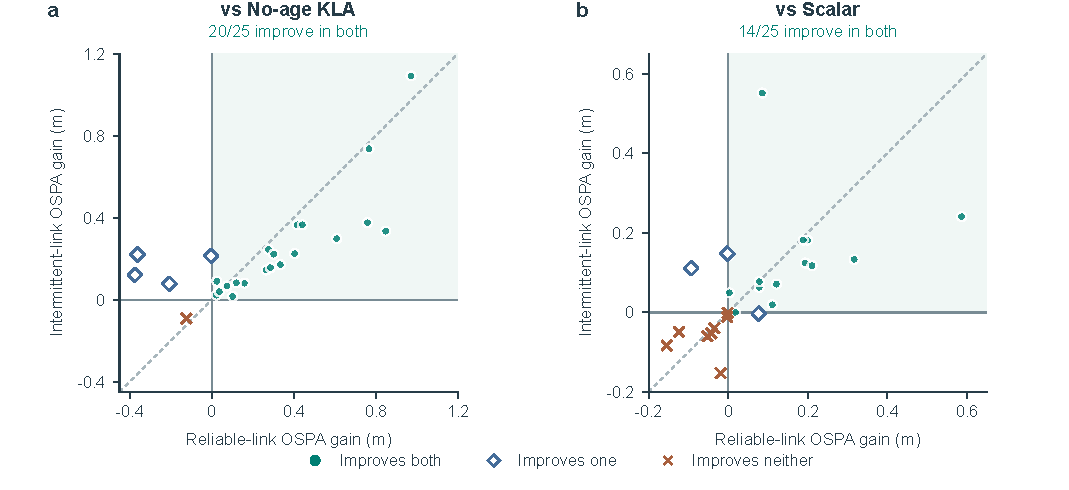
\includegraphics[width=\textwidth]{figures/gaussian_paired.pdf}
 \caption{Complete 25-sequence comparisons. Small dots are individual
 sequence OSPA differences, GCE minus the labeled control; large points
 and bars show equal-sequence means and 95\% percentile intervals from
 10,000 sequence resamples. Negative values favor GCE. All points and
 both link conditions are included; intervals describe this development
 corpus.}
 \label{fig:paired}
\end{figure*}

Both missed-target and false-target squared costs decrease relative to
No-age KLA and Recency. Against No-age KLA, mean missed cost decreases
by \MissGainNoAgeReliable\%/\MissGainNoAgeIntermittent\%, and false cost
by \FalseGainNoAgeReliable\%/\FalseGainNoAgeIntermittent\%
(reliable/intermittent). On common matched truth, GCE/No-age RMSE is
\LocMainNoAgeReliable/\LocNoAgeReliable\ m with reliable links and
\LocMainNoAgeIntermittent/\LocNoAgeIntermittent\ m with intermittent
links, on \SupportNoAgeReliable\ and \SupportNoAgeIntermittent\
instances. The lower set error therefore does not arise solely from
trading worse localization for a different target count.

GCE also has lower sequence-macro OSPA than MIL-AM and both TC windows
in both conditions. These are comparisons with the stated adaptations;
TC's separate local-track architecture and MIL's arithmetic pooling
differ from recursive geometric density fusion. The controlled
No-age, Recency, and Scalar comparisons more directly isolate the change
to the fusion rule.

\subsection{The contribution of joint normalization}
The complete Scalar control obtains \ScalarReliable/\ScalarIntermittent\
m OSPA. The paired GCE-minus-Scalar differences are \DeltaScalarReliable\ m
[\DeltaScalarLowReliable, \DeltaScalarHighReliable] and
\DeltaScalarIntermittent\ m
[\DeltaScalarLowIntermittent, \DeltaScalarHighIntermittent].
Here differences retain the GCE-minus-control convention; both intervals
lie below zero. GCE also lowers common-target RMSE from
\LocScalarReliable\ to \LocMainScalarReliable\ m and from
\LocScalarIntermittent\ to \LocMainScalarIntermittent\ m.
Relative to Scalar, the correction reduces mean missed cost while
slightly increasing mean false cost, as shown in
Table~\ref{tab:ablation}.

\begin{table*}[t]
\centering\small
\caption{Ablations of the recursive tracker. Each w/o row removes one GCE component; Scalar is a separate existence-only reference. Units and boldface follow Table~\ref{tab:main}.}
\label{tab:ablation}
\setlength{\tabcolsep}{6pt}
\begin{tabular*}{\textwidth}{@{\extracolsep{\fill}}lrrrrrr@{}}
\toprule
& \multicolumn{3}{c}{Reliable links} & \multicolumn{3}{c}{Intermittent links} \\
\cmidrule(lr){2-4}\cmidrule(lr){5-7}
Method & OSPA & Missed & False & OSPA & Missed & False \\
\midrule
Scalar reference & 3.526 & 78.625 & \textbf{34.536} & 3.832 & 86.342 & \textbf{40.523} \\
\midrule
w/o curvature guard & 3.491 & 74.845 & 35.376 & 3.805 & 84.047 & 41.615 \\
w/o history switch & 3.467 & 70.282 & 38.148 & 3.776 & 80.266 & 43.105 \\
w/o score constraint & 3.713 & \textbf{55.993} & 59.014 & 3.922 & \textbf{69.042} & 57.784 \\
\midrule
\textbf{GCE (complete)} & \textbf{3.456} & 71.095 & 36.303 & \textbf{3.761} & 80.344 & 41.971 \\
\bottomrule
\end{tabular*}
\end{table*}


To distinguish immediate fusion effects from changes accumulated through
recursive filtering, we also re-extract estimates on GCE's saved fusion
inputs. Using the old spatial pool and Scalar existence gives OSPA
\FixedScalarReliable/\FixedScalarIntermittent\ m on actual fusion
frames, versus \FixedMainReliable/\FixedMainIntermittent\ m for the
joint correction. Replacing only the mean or only the existence gives
intermediate diagnostics. These substitutions do not reproduce the
Scalar trajectory: the larger full-run difference also includes later
association, pruning, and extraction effects.

\subsection{What the guards and history term contribute}
Figure~\ref{fig:components} and Table~\ref{tab:ablation} report every
declared component removal. Omitting the curvature guard raises mean
OSPA in both conditions; its paired interval excludes zero only with
intermittent links. The unguarded version encounters two nonintegrable
aggregates under reliable links, which trigger the shared fallback.
GCE encounters none. The largest observed immediate position changes
are 6.85/7.93 m for GCE, versus 28.68/49.62 m without the source guard.
These observed maxima illustrate the effect of rejecting unsuitable
Gaussian ratios; they are not error bounds.

\begin{figure*}[t]
 \centering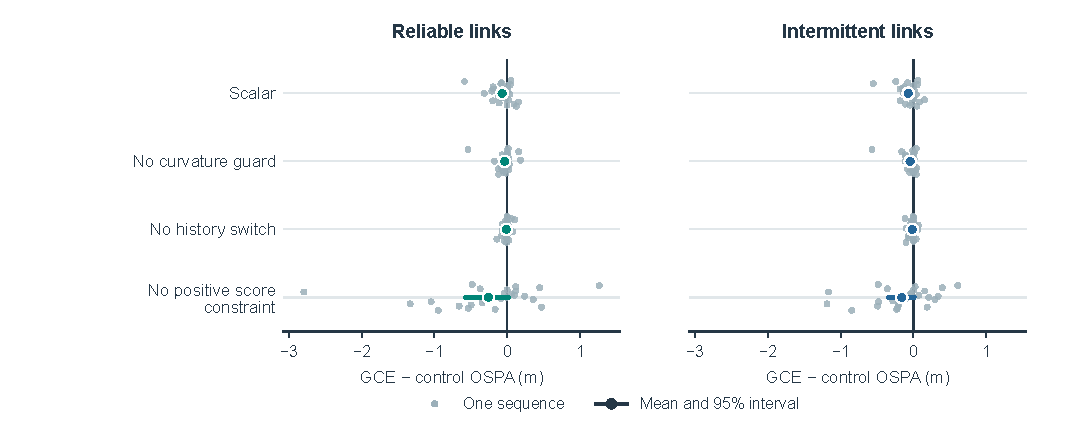
\includegraphics[width=\textwidth]{figures/gaussian_components.pdf}
 \caption{Component evidence on all 25 sequences. GCE-minus-control OSPA
 differences use the same point and interval conventions as
 Fig.~\ref{fig:paired}. The Scalar control removes the spatial ratio;
 the other controls remove one admission or base-weighting component.
 Intervals crossing zero do not establish an OSPA contribution for that
 component.}
 \label{fig:components}
\end{figure*}

Removing the conservative history switch changes mean OSPA by only
about 0.01 m, and both intervals include zero. Removing the positive
score constraint substantially increases mean false-target cost but
reduces missed-target cost. Its total OSPA intervals also include zero.
Thus the current experiment supports the full rule and the joint
correction over Scalar, while leaving some individual design choices
only weakly resolved.

\subsection{Development results and the common local model}
On the nine-sequence development subset, GCE attains
\DevMainReliable/\DevMainIntermittent\ m OSPA, compared with
\DevNoAgeReliable/\DevNoAgeIntermittent\ m for No-age KLA and
\DevScalarReliable/\DevScalarIntermittent\ m for Scalar.
All fixed methods and both conditions are retained in the accompanying
source data. The development Scalar comparison is weaker than the
25-sequence result: its two intervals include zero.

The score-aware local model itself matters. In the 25-sequence
evaluation, unmarked No-age KLA has OSPA
\UnmarkedNoAgeReliable/\UnmarkedNoAgeIntermittent\ m, compared with
\NoAgeReliable/\NoAgeIntermittent\ m when both methods use the common
score-aware update. That gain belongs to the local observation model.
The additional GCE improvement is measured against the latter, and the
no-positive-score-constraint ablation retains that same local model.

\subsection{Actual communication cost}
Table~\ref{tab:communication} and Fig.~\ref{fig:communication} use the
native zero-vector codec for GCE. It reproduces every primary trajectory
and all original local and fusion diagnostics under both link conditions.
Across the 25 sequences, raw payload falls by
\CodecRawSavingReliable\%/\CodecRawSavingIntermittent\% relative to
the full 352-byte Gaussian representation; fragmented totals fall by
\CodecWireSavingReliable\%/\CodecWireSavingIntermittent\%.

\begin{table*}[t]
\centering\small
\caption{Mean actual MiB per sequence over 25 sequences. GCE uses the exact zero-vector codec. Fragmented totals include attempted packet fragments and modeled control traffic; delivered raw bytes count successful deliveries only.}
\label{tab:communication}
\setlength{\tabcolsep}{6pt}
\begin{tabular}{lrrrrrr}
\toprule
& \multicolumn{3}{c}{Reliable links} & \multicolumn{3}{c}{Intermittent links} \\
\cmidrule(lr){2-4}\cmidrule(lr){5-7}
Method & Raw & Delivered & Fragmented & Raw & Delivered & Fragmented \\
\midrule
Local & 0.000 & 0.000 & 0.000 & 0.000 & 0.000 & 0.000 \\
MIL-AM & 6.241 & 6.241 & 10.205 & 5.858 & 4.163 & 10.020 \\
TC-5 & 1.136 & 1.136 & 7.056 & 1.136 & 0.779 & 7.056 \\
TC-10 & 2.223 & 2.223 & 7.234 & 2.223 & 1.521 & 7.234 \\
No-age KLA & 3.890 & 3.890 & 8.347 & 3.882 & 2.748 & 8.294 \\
Recency & 3.591 & 3.591 & 8.139 & 3.650 & 2.575 & 8.103 \\
Conservative & 3.686 & 3.686 & 8.228 & 3.717 & 2.630 & 8.248 \\
Capped-score & 3.803 & 3.803 & 8.283 & 3.810 & 2.690 & 8.286 \\
Capped-cal. & 3.745 & 3.745 & 8.251 & 3.790 & 2.673 & 8.253 \\
Scalar & 3.727 & 3.727 & 8.190 & 3.886 & 2.738 & 8.322 \\
\textbf{GCE} & 4.562 & 4.562 & 8.687 & 4.717 & 3.338 & 8.878 \\
GCE full Gaussian packet & 5.724 & 5.724 & 9.788 & 5.978 & 4.219 & 9.951 \\
\bottomrule
\end{tabular}
\end{table*}


\begin{figure*}[t]
 \centering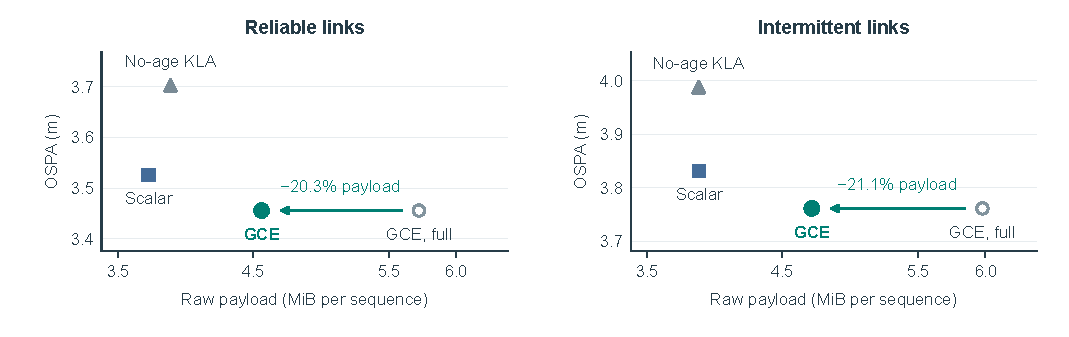
\includegraphics[width=\textwidth]{figures/gaussian_communication.pdf}
 \caption{Actual mean MiB per sequence over 25 sequences. Raw payload and
 fragmented totals compare No-age KLA, Scalar, and two GCE packet formats.
 Full Gaussian and exact zero-vector GCE packets yield identical tracking
 trajectories. Fragmented totals include modeled control traffic and use
 16,384-byte fragments. The delivery trace is fixed across methods.}
 \label{fig:communication}
\end{figure*}

Compared with No-age KLA, GCE's compressed raw payload is still
\CodecRawExtraNoAgeReliable\%/\CodecRawExtraNoAgeIntermittent\% larger,
while fragmented cost is
\CodecWireExtraNoAgeReliable\%/\CodecWireExtraNoAgeIntermittent\% larger.
The gain therefore trades additional transmitted information for lower
tracking error. The 16,384-byte fragmentation model makes byte savings
discontinuous at packet boundaries. We do not infer real-network latency,
throughput, or size-dependent loss from this fixed delivery trace.
